%
% skript.tex -- Lecture notes for the PartDiff lectures given at the
%               MSE Master
%
% (c) 2006-2018 Prof. Dr. Andreas Mueller, HSR
%
\documentclass[a4paper,12pt]{book}
\usepackage[utf8]{inputenc}
\usepackage[T1]{fontenc}
%\usepackage{german}
\usepackage{times}
\usepackage{geometry}
\geometry{papersize={210mm,297mm},total={160mm,240mm},top=31mm,bindingoffset=15mm}
\usepackage{amsmath}
\usepackage{amssymb}
\usepackage{amsfonts}
\usepackage{amsthm}
\usepackage{amscd}
\usepackage{graphicx}
\usepackage{fancyhdr}
\usepackage{textcomp}
\usepackage{txfonts}
\usepackage[all]{xy}
\usepackage{paralist}
\usepackage[colorlinks=true]{hyperref}
\usepackage{array}
\usepackage{tikz}
\usepackage{pdfpages}


\usepackage{pdflscape}

%figure float
\usepackage{float}

%bibliography
\usepackage[hyperref=true,backend=biber,style=ieee,defernumbers=true]{biblatex}
\addbibresource{references.bib}

\input{common/linsys.tex}
\makeindex


\begin{document}
\pagestyle{fancy}
\lhead{}
\rhead{}
\frontmatter
\newcommand\HRule{\noindent\rule{\linewidth}{1.5pt}}



\hypersetup{
	colorlinks=true,
	linktoc=all,
	linkcolor=blue
}


\newtheorem{satz}{Theorem}[chapter]
\newtheorem{problem}[satz]{Problem}
\newtheorem{hilfssatz}[satz]{Lemma}
\newtheorem{definition}[satz]{Definition}
\newtheorem{annahme}[satz]{Assumption}
\newtheorem{aufgabe}[satz]{Task}
\newenvironment{beispiel}[1][Example]{%
	\begin{proof}[#1]%
		\renewcommand{\qedsymbol}{$\bigcirc$}
	}{\end{proof}}
%\allowdisplaybreaks


\begin{titlepage}
\vspace*{\stretch{1}}
\HRule
\vspace*{10pt}
\begin{flushright}
{\Huge
Low Power WakeUp-Receiver}

%\Large{with Rotation, GPS and On-Board-Diagnostics Sensor Data}
\end{flushright}
\begin{flushright}
{\Large Project Electrical Engineering AS2019}
\end{flushright}
\HRule

\vspace{70pt}
\large
\textbf{Authors}

Cédric Renda, Manuel Tischhauser

\textbf{Supervisor}

Prof. Dr. Heinz Mathis

\textbf{Assistant Supervisor}

Selina Malacarne

\textbf{Subject}

Wireless Communications



\vspace*{\stretch{2}}
\begin{center}
HSR Hochschule Für Technik Rapperswil

\today
\end{center}
\end{titlepage}


\chapter*{Abstract}

\section*{Introduction}
In company buildings, universities and other similar facilities, it is usual to attach occupancy schedules next to a room entrance. These schedules are most of the time printed on paper, or in more modern buildings, displayed on a screen. Using paper, it is impracticable to take short-term changes into account, since every adjustment needs to be made by printing a new schedule. Hence, screens need to be connected to the power grid, which entails extensive installation work, or powered by a battery, which needs to be replaced from time to time. All these disadvantages could be avoided by using a screen which harvests its energy from the indoor lightning, and is updated via a wireless interface.



\section*{Approach}
The system is powered by a energy storage system that uses solar cells to harvest energy. This energy will then be stored in a super-capacitor to ensure minimal power leakage. As this specific type of energy harvesting unit cannot provide vast amounts of energy over a longer time period, the whole system fully runs in short bursts. One solution introduced to save energy is by using an E-Paper Display (EPD). The EPD only uses energy when updating its screen but not for maintaining, the image displayed on the screen, which results in a high energy reduction.   Furthermore, in addition to the EPD a constantly listening ultra-low power wakeup receiver is used. This will further enhance the system, as it will generate an interruption to enable the power supply of the remaining system only when receiving a specific wakeup sequence. The remaining part then receives data via Bluetooth, which will then display the data and eventually cuts its own power supply to enter a new cycle of low-power listening mode.

\section*{Conclusion}
This semester thesis was designed to elaborate a sustainable screen in order to display a room’s occupancy next to its entrance. Upon analysis of potential solutions, it can be concluded that the outlined energy harvesting does provide enough energy to sustainable run the introduced E-Paper Display (EPD), if up-dating the schedule does not occur too frequently. Moreover, it has been identified that a wakeup receiver is the most suitable tool to support the display. The implementation of a latch circuit makes it possible to switch off the whole system (except for the wakeup receiver) when not in usage. In total the wakeup receiver consumes a maximum of $4.5\,\mu \text{W}$ during listening mode while the system harvests around $485,52\,\mu\text{W}$. 
\tableofcontents




\mainmatter

\chapter*{Abbreviations}
\addcontentsline{toc}{chapter}{Abbreviations} 
%A
\begin{acronym}
	\acro{ask}[ASK]{Amplitude Shift Keying}
\end{acronym}

%B
\begin{acronym}
	\acro{ble}[BLE]{Bluetooth Low Energy}
\end{acronym}

%F
\begin{acronym}
	\acro{fifo}[FIFO]{First In First Out}
\end{acronym}

\begin{acronym}
	\acro{fram}[FRAM]{Ferroelectric Random Access Memory}
\end{acronym}

%G
\begin{acronym}
	\acro{gpio}[GPIO]{General Purpose Input/Output}
\end{acronym}

\begin{acronym}
	\acro{gui}[GUI]{Graphical User Interface}
\end{acronym}

%H
\begin{acronym}
	\acro{hsr}[HSR]{Hochschule für Technik Rapperswil}
\end{acronym}

%I
\begin{acronym}
	\acro{fraun}[IIS]{Fraunhofer-Institut für Integrierte Schaltungen}
\end{acronym}

\begin{acronym}
	\acro{iot}[IoT]{Internet of Things}
\end{acronym}

%O
\begin{acronym}
	\acro{ook}[OOK]{On-Off Keying}
\end{acronym}

%S
\begin{acronym}
	\acro{spi}[SPI]{Serial Peripheral Interface}
\end{acronym}

%T
\begin{acronym}
	\acro{ttl}[TTL]{Transistor-Transistor Logic}
\end{acronym}

%U
\begin{acronym}
	\acro{uart}[UART]{Universal Asynchronous Receiver Transmitter}
\end{acronym}

\begin{acronym}
	\acro{usb}[USB]{Universal Serial Bus}
\end{acronym}










\lhead{Introduction}
\chapter{Introduction}

\section{RealPower System}

\chapter{Theory}

\section{E-Paper Display}
There are several different technologies which are applied in e-paper displays.
But since the developed prototype uses a microencapsulated electrophoretic display, this section only describes this specific implementation.

A film, consisting of microscopic capsules, is coated onto a backplane, which basically is a matrix of electrodes.
On top of that comes a common electrode, called the frontplane.
This setup is shown in figure \ref{theory:capsules}.

\begin{figure}[h]
	\centering
	\includegraphics[width=0.9\textwidth]{2-theory/e-paper-display/graphics/capsules.pdf}
	\caption{filler pic\label{theory:capsules}}
\end{figure}

Each capsule in the film itself contains a transparent fluid and particles of two opposite charges.
One type of particle scatters the light while the other one absorbs it.
The particles now begin to move in opposite directions thought the fluid when exposed two a electrical field. 
The pixel (defined by the electrode size) appears white if the scattering particles ar near the frontplane and black if otherwise.
If no voltage is applied to the electrodes, the particles maintain their last position.
This makes it possible to switch of the power supply when no image update is needed which is the reason why the power consumption is strongly reduced compared to other types of display \cite{amundson}.

\begin{figure}[h]
	\centering
	\includegraphics[width=0.9\textwidth]{2-theory/e-paper-display/graphics/epaper_mikroskop.pdf}
	\caption{E-paper display under microscope with 250x magnification\label{theory:micro}}
\end{figure}

Figure \ref{theory:micro} shows a e-paper display with 250x magnification.
One electrode is coated by many capsules, which are between 0.02 mm and 0.04 mm in diameter.

\section{Wakeup Receiver}
To safe power with a conventional receiver, it needs to be programmed in such a way, that it is kept in a sleep mode.
To check if any data was sent, it needs to wake up periodically to check for notifications.
To set this duty cycle is a trade off between response time and power consumption.
Is the period longer, the receiver is also a longer time in its sleep mode.
This period defines also directly the response time, since data can only be received in the running mode.
A wakeup receiver now allows a device to be constantly in listening mode, while consuming low energy.
Added to the system, the actual microcontroller, which coordinates the data transmission and other tasks, stays shut down with only the wakeup receiver in listening mode.
After receiving a defined pattern over this channel, the wakeup receiver generates an interrupt to wake up the microcontroller. 
It can now establish a channel over a different wireless module or execute another task.
When done, the microcontroller puts itself and all other modules except the wakeup receiver in sleep mode again.
Figure \ref{theory:wake} shows a comparison of both the conventional approach and the solution with the wakeup receiver. 
\begin{figure}[ht]
	\centering
	\includegraphics[width=0.9\textwidth]{2-theory/wakeup/graphics/wake_comp.pdf}
	\caption{Top: Microcontroller checks periodically for incoming data. Bottom: Constantly listening  wakeup receiver.\label{theory:wake}}
\end{figure}
One can argue that the wakeup receiver module consumes in general more power, than the microcontroller in sleep mode.
But since the microcontroller only wakes up when a task needs to be done, the overall energy consumption (area underneath the curves summarized) is going to be smaller if the occurring wakeup event comes infrequently or over longer periods of time.
The response time can be kept in the microsecond range.

\section{software grafik zeichen}
\chapter{Evaluation}
This chapter lists the pros and cons of available Technologies.
On this basis was evaluated, which hardware is suitable.

\section{Wakeup Receiver}
In this semester thesis, two different implementations of the wakeup receiver technology were compared.
The AS3933 from AMS and the RFicient from the \acf{fraun} which kindly provided an evaluation kit before the actual release of the product.
This section first introduces both products, before comparing them with a series of tests in a for this application realistic environment.

\subsection{AS3933}
The AS3933 is a low frequency wakeup receiver, which uses \acs{ask} to modulate a carrier frequency between 15-150\,kHz.
The transmitter sends a manchester encoded, programmable wakeup pattern of length 16 or 32 bit.
If this pattern is detected on the receiver end, a wakeup interrupt is generated.
It is also possible to disable the the pattern decoder to run the chip in a frequency detection mode, where a wakeup interrupt is generated as soon as any pattern on the specified frequency is received.
More important features on the receiver end are:
\begin{itemize}
	\item[-] Receiver sensitivity $80\,\mu\text{V$_{\text{RMS}}$}$
	\item[-] Current consumption in 3-channel listening mode $2.3\,\mu\text{A}$
	\item[-] Operating supply range $2.4\,\text{V}-3.6\,\text{V}$
	\item[-] Three antennas (enables 3D detection)
	\item[-] Channels  individually selective to reduce power consumption
\end{itemize}
The low power consumption makes it possible run the receiver in listening mode below $8.3\,\mu\text{W}$\cite{as3933}.

The demo kit comes with a \acs{gui}, which enables the user to set the parameters as desired.

\subsection{RFicient}
The Rficient from the \acs{fraun} uses \acs{ook} to modulate a 868\,MHz signal.
It can either run in pure wakeup mode, where the receiver generates an interrupt as soon as a code is received or a selective mode, where a 16 bit wakeup preamble needs to match the receiver. 
After the preamble is detected, the data rate can be changed to transfer more bits which can be sent over an \acs{spi}-bus to a connected device.
This way, it is possible to transmit data bits after the actual wakeup.
Data rates can be set in a range between $256\,\text{bp/s}-32\,\text{kbp/s}$.
The most important features are:
\begin{itemize}
	\item[-] Receiver sensitivity -80\,dBm
	\item[-] Energy consumption $3\,\mu\text{A}$ at $1.5\,\text{V}$ (data rate 1 kbit/s)
	\item[-] Unidirectional data transfer possible	
\end{itemize}
The power consumption therefore is in listening mode (data rate = 1 kb/s) $4.5\,\mu\text{W}$.

Just as the AS3933, the RFicient demo kit comes with a \acs{gui}, which enables the user to set the important parameters and even access the register directly \cite{rficient}.

\subsection{Test run in realistic environments}
It is not easy to compare the two wakeup receivers directly, since one operates in the 

\begin{figure}[ht]
	\centering
	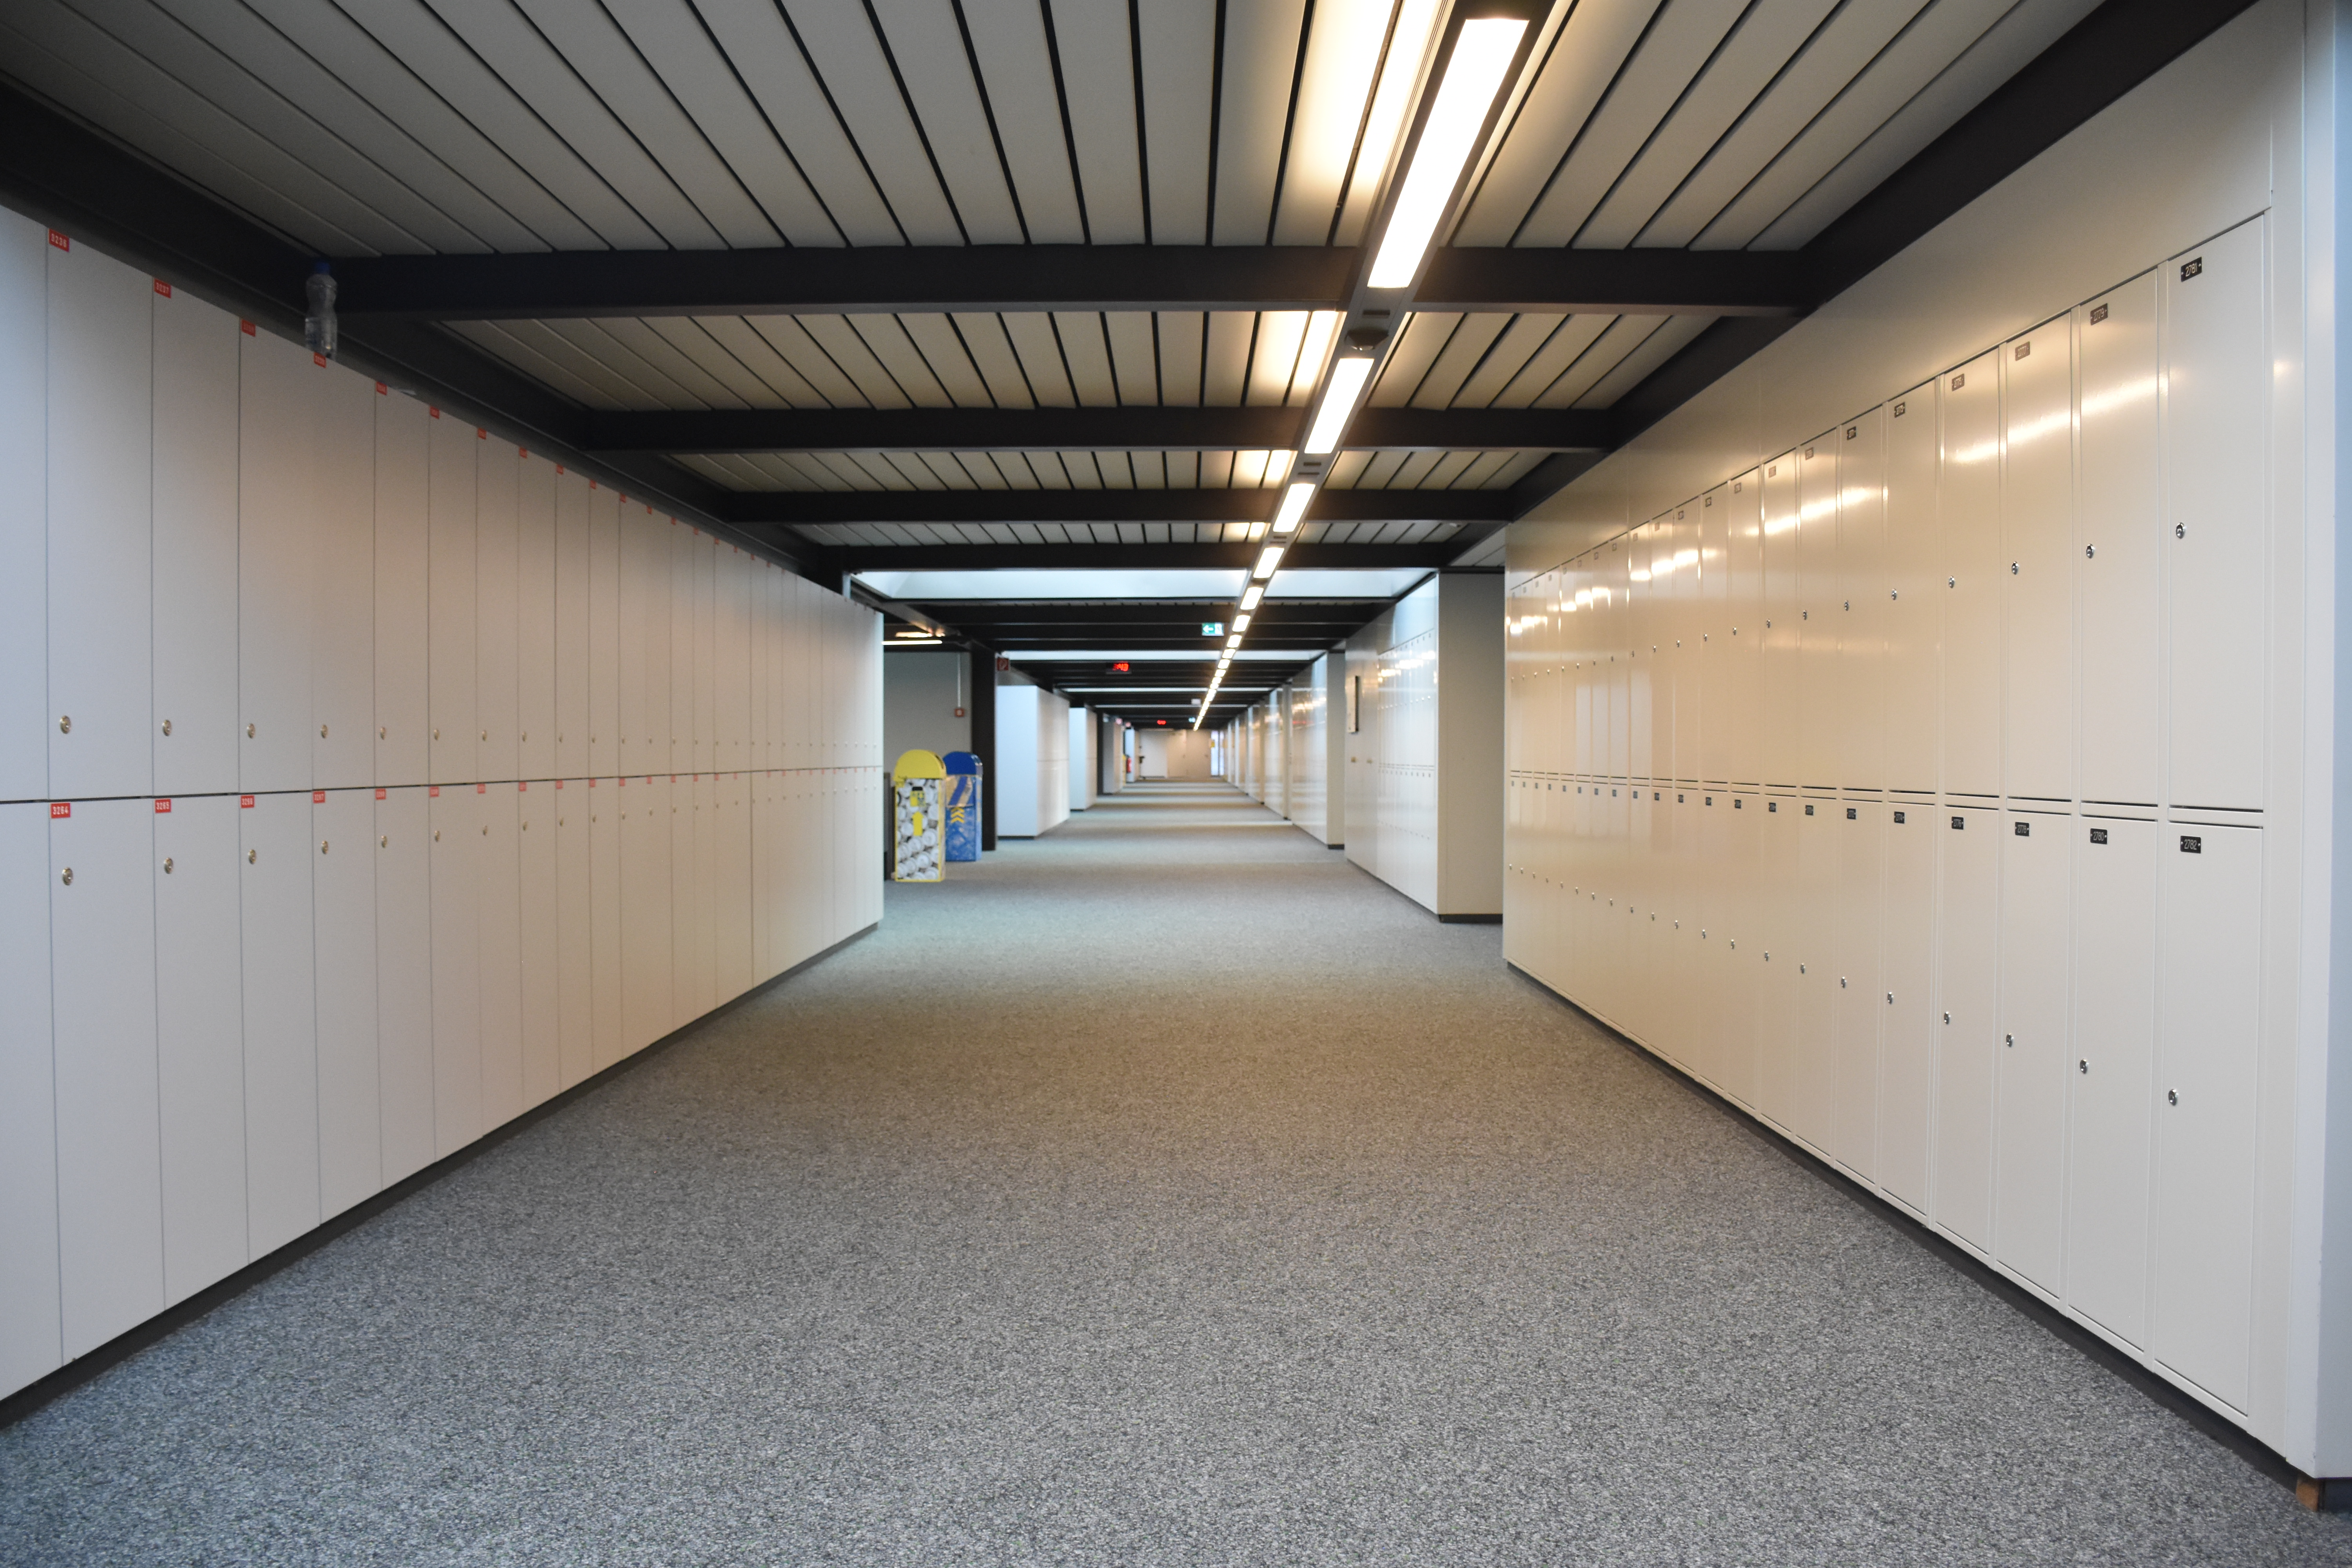
\includegraphics[width=0.9\textwidth]{3-evaluation/graphics/env1.jpg}
	\caption{Test environment 1 (filler)\label{evaluation:env1}}
\end{figure}

\begin{figure}[ht]
	\centering
	\includegraphics[width=0.9\textwidth]{3-evaluation/graphics/env2.jpg}
	\caption{Test environment 2 (filler)\label{evaluation:env2}}
\end{figure}
\chapter{Development}

\section{Overview}


\textbf{Not Up To Date Graphic}\\

\includegraphics[scale=0.5]{5-development/overview/graphics/Blockschaltbild.pdf}


\section{Hardware}
\subsection{Energy Harvesting}
The Screen should be self-sufficient, thus some sort of Energy-Harvesting unit is needed.
It was apparent to choose light as the energy source, since the screen will be used in rooms, which are most of the day artificially illuminated.
A power management chip converts the energy  obtained by solar cells to a suitable voltage.
This way, a super-capacitor, which is used as an energy storage device is charged.

\subsubsection{Solar cell}
The AM-1522 by Panasonic was chosen as the solar cell.
One panel has a area of 55.0 mm $\times$ 40.5 mm and delivers up to 58.7 $\mu\text{A}$ when operating at an optimal voltage of 2.1V, provided an Illumination of 200 lux.
To keep a reasonable display to panel ratio, four cells where used in parallel, which corresponds to an area of ca. 89.1 cm$^2$ (Display area = 283 cm$^2$). Therefore, the solar cells should provide a power of

\begin{align}
	P = U\cdot I = 4\cdot 57.8\ \mu\text{A}\cdot 2.1\ \text{V}=485.52\ \mu \text{W},\label{development:cell_power}
\end{align}

given a 200 lux illumination. \cite{amorton}

\subsubsection{Power management}
The ADP5090 from Analog Devices was used in the power management.
This boost regulator makes it possible to charge storage elements, such as rechargeable batteries and super capacitors with the input dc-power provided by the PV-cell.

Utilized features are:
\begin{itemize}
	\item[-] Maximum power point tracking
	\item[-] Efficiency up to 90\%
	\item[-] Input voltage $V_{in}$ from 80 mV to 3.3 V
	\item[-] Programmable voltage range (2.2 V to 5.2 V) for the storage element
\end{itemize}

To prevent the storage element from overdischarging, the ADP5090 enables the user to set a maximal Voltage with resistors:

\begin{align}
	V_{BAT\_TERM} = \frac{3}{2}\cdot V_{REF}\cdot\left(1+\frac{R_{TERM1}}{R_{TERM2}} \right).\label{development:v_bat_term} 
\end{align} 

The same procedure is applied to set a minimal Voltage:

\begin{align}
	V_{BAT\_SD}=V_{REF}\cdot \left(1+\frac{R_{SD1}}{R_{SD2}} \right).\label{development:v_bat_sd} 
\end{align}  

While discharging, the ADP5090 will switch off the output $V_{SYS}$ if $V_{BAT\_SD}$ is reached. This prevents the storage element from overdischarging.
The output voltage $V_{SYS}$, where the load is attached, will therefore always stay in this programmed range $(V_{BAT\_SD}\le V_{SYS}\le V_{BAT\_TERM})$.
\cite{adp}

\subsubsection{Super capacitor}
As energy Storage, a super capacitor from Taiyo Yuden has proven to be suitable.
The LIC1235RS3R8406 is a 40 F cylinder type lithium ion capacitor.
It's operating voltage range is between 2.2 V and 3.8 V.
Discharging the capacitor lower than 2.2 V causes shorter lifetime and higher leakage.
the same applies to charging the capacitor over 3.8 V.
\cites{yuden}

\subsubsection{Combined test}
To test the behaviour of the power management, supercapacitor and solar cells, a couple of measurements were executed.
The input voltage from the solar cells ($V_in$), voltage of the supercap ($V_{BAT}$) and the output voltage ($V_{SYS}$) were tracked. Additionally, the illuminance near the PV-cells ($E_v$) was recorded.

To carry out the measurement, it was first necessary, to adjust the minimal and maximal voltage of the ADP5090.

\begin{figure}[h]
	\centering
	\includegraphics[width=0.9\textwidth]{5-development/hardware/graphics/laden.pdf}
	\caption{Charging behaviour\label{development:charge}}
\end{figure}

\begin{figure}[h]
	\centering
	\includegraphics[width=0.9\textwidth]{5-development/hardware/graphics/entladen.pdf}
	\caption{Discharging behaviour\label{development:discharge}}
\end{figure}

\section{Software}
\begin{figure}[ht]
	\centering
	\includegraphics[width=0.9\textwidth]{4-development/software/graphics/1.png}
	\caption{not up to date sequence\label{software:sequence}}
\end{figure}

The software of the ULPWUR is separated in three different parts. 

\includegraphics[scale=0.3]{4-development/software/graphics/font12.pdf}

\subsection{Receiver}

\subsubsection{Python-script}
\lstset{basicstyle=\footnotesize}
\lstdefinestyle{mystyle}{
	language=Python,
	basicstyle=\footnotesize\ttfamily,
	morekeywords={as},
	keywordstyle=\color{blue!50!black},
	stringstyle=\color{green!50!black},
	numberstyle=\color{red},
	emph={int,char,double,float,range, len},
	emphstyle=\color{violet}
}
\lstset{style=mystyle}

A short python script enables the user to send the data to the display.
This script is looked at here little by little.

%\begin{enumerate}
	%\item Include of the needed packages open a port to the nRF52480 development kit.
	\begin{lstlisting}
		import serial
		import time
		
		baudrate = 115200
		com_port = 'COM14'
		
		device = serial.Serial(com_port, baudrate, writeTimeout=0)
	\end{lstlisting}
	 
%\end{enumerate}


\subsubsection{nRF52840}
The software on both sides of the bluetooth channel is very similar, thus it is explained in this section.
A \acs{ble} example project, which was provided by nordic, was only slightly changed to fit the purpose of this prototype.

Before a connection is established, the module on the receiver side is known as peripheral, and the module on transmitter end as the central device.
After the receiver is woken up with the RFicient, the peripheral starts advertising.
Advertising basically means sending data packets periodically with information for the central device.
The central is scanning for the this advertisement and can based on this information decide, if it wants to connect.
Is the connection established, it is now possible to exchange data through this channel.
This process is illustrated in figure \ref{software:ble}.
\begin{figure}[ht]
	\centering
	\includegraphics[width=0.9\textwidth]{4-development/software/graphics/ble.pdf}
	\caption{\acs{ble}-communication with the nRF52480\label{software:ble}}
\end{figure}

The central serves after connection as the client.
It can make read and write requests to access the data on the peripheral, which acts as the server.
The server on the other hand can only send notifications to the client if new data is ready.
It should be noted, that the roles of client and server do not in any case have to be assigned to the central and peripheral, but also the other way around. 

\subsection{Transmitter}


\chapter{Results}

\section{Power consumption}
\subsection{Power measurement}
To look at the energy consumption in detail, the N6705B power analyzer from keysight was used as the power supply.
To carry out measurements, the ADP5090 with the solar cells and super cap was disconnected and the remaining components connected to the power analyser with a fixed voltage of 3.3\,V.
This way, the voltage and current over one write-cycle could be tracked.
The result is plotted in Figure \ref{results:ui}.
\begin{figure}[ht]
	\centering
	\includegraphics[width=0.9\textwidth]{5-results/energy/logger/ui.pdf}
	\caption{Current and Voltage during one write-cycle.\label{results:ui}}
\end{figure}
One write-cycle takes about 5.8 seconds.
In this interval, the STM32, nRF52480 and display driver are active.
Clearly visible is the current peak which occurs when the system is woken up.
Short after the 5 seconds mark, initializing and data receiving is finished and the display is refreshed.
The current peaks there are due to the charge pumps on the display driver.

With voltage and current given, the power over time can be calculated.
This curve is plotted in Figure \ref{results:p}.
The power follows obviously the same course like the current since the voltage is constant.
\begin{figure}[ht]
	\centering
	\includegraphics[width=0.9\textwidth]{5-results/energy/logger/p.pdf}
	\caption{Power consumption during one write cycle.\label{results:p}}
\end{figure}
The energy needed for one write-cycle is given with the integral of the power over time:
\begin{align}
	E = \int_{0}^{8\,\text{s}}P(t)\text{dt}\approx 2.7504\,\text{J}\label{result:energy}.
\end{align}
Like stated in \eqref{development:cell_power} the solar cells provide $485.52\,\mu \text{W}$ at 200\,lux.
Considering the Rficient which consumes $4.5\mu \text{W}$, it is possible to estimate the time needed, to harvest the power for one write cycle:
\begin{align}
	t_{\text{E}}=\frac{2.7504\,\text{J}}{485.52\,\mu \text{W}-4.5\mu \text{W}}=5717.85\,\text{s}\approx 1\,\text{h } 35\,\text{min}.
\end{align}
Not taken into account is the leakage of the super capacitor and losses in the ADP5090.

\subsection{Energy storage}
The stored energy in a capacitor is
\begin{align*}
	E =\frac{1}{2}CU^2.
\end{align*}
since the capacitor operates between 2.2\,V and 3.6\,V, the total stored energy is
\begin{align}
	E_{\text{ges}} = \frac{1}{2}C(U_{\text{max}}^2-U_{\text{min}}^2)=\frac{1}{2}\cdot 40\,\text {F}\cdot((3.6\,\text{V})^2-(2.2\,\text{V})^2)=162.4\,\text{J}\label{result:store}.
\end{align}
If again the loss in the ADP5090 and the leakage of the super cap is neglected, it is possible to estimate the time
\begin{align}
	t_{\text{func}}=\frac{162.4\,\text{J}-2.7504\,\text{J}}{4.5\,\mu\text{W}}=3.54877\cdot 10^{-7}\,\text{s}\approx 411\,\text{d}
\end{align} 
in which the prototype is fully functional when no energy is harvested.
The 2.7504\,J are subtracted, because on should be able to refresh the display after this time.
This result should be taken with caution, because it neglects losses and does not consider the tolerance of the capacitor ($\pm20\%$ corresponds to $\pm8\,\text{F}$ with a 40\,F capacitor \cite{yuden}).
The order of magnitude tough should be correct.

\subsection{Amount of display refreshes}
With the results from the Equations \eqref{result:energy} and \eqref{result:store}, the amount of display refreshes can be calculated:
\begin{align}
	n = \left\lfloor\frac{162.4\,\text{J}}{2.7504\,\text{J}}\right\rfloor=59.
\end{align}
Not that in this calculation, additional charging is neglected and the super capacitor is fully charged.

To verify this value, the super cap was charged to 3.5\,V and the whole refresh sequence was repeated until the voltage reached 2.2\,V.
Under this conditions, the display could be refreshed 46 times.

\chapter{Summary}

\section{Conclusion}
In the course of this thesis, a working prototype of a occupancy schedule was developed.
y

\section{Future work}
Following improvements on the prototype have to be made, before developing a complete layout of the receiver:
\begin{itemize}
	\item[-] Developing a power management which protects the super capacitor from over discharging
	\item[-] Changing the microcontroller to display driver connection from \acs{spi} to a parallel bus (for ex. I80)
	\item[-] Synchronising of the refresh sequence on transmitter end
\end{itemize}
These adjustments should ensure functionality and reduce power consumption of the prototype.

Further it may be useful, to extend the \acs{ble}-communication to a mesh network, or even change to a different protocol with more range.






%bibliography
\chapter*{Sources}
\addcontentsline{toc}{chapter}{Sources} 
\printbibliography[heading=none]

\appendix
\chapter{Requirements}

\newpage

\section{Assignment}
\begin{figure}[H]
	\centering
	\includegraphics[trim= 0cm 0cm 0cm 0cm,page=1,width=16cm]{../Aufgabenstellung/LowPowerWakeupReiceiver.pdf}
\end{figure}
\begin{figure}[H]
	\centering
	\includegraphics[trim= 0cm 0cm 0cm 0cm,page=2,width=16cm]{../Aufgabenstellung/LowPowerWakeupReiceiver.pdf}
\end{figure}

\newpage
\section{Requirement Specification}
\begin{figure}[H]
	\centering
	\includegraphics[trim= 0cm 0cm 0cm 0cm,page=1,width=16cm]{../Pflichtenheft/HSR_SRS_main.pdf}
\end{figure}
\begin{figure}[H]
	\centering
	\includegraphics[trim= 0cm 0cm 0cm 0cm,page=2,width=16cm]{../Pflichtenheft/HSR_SRS_main.pdf}
\end{figure}
\begin{figure}[H]
	\centering
	\includegraphics[trim= 0cm 0cm 0cm 0cm,page=3,width=16cm]{../Pflichtenheft/HSR_SRS_main.pdf}
\end{figure}
\begin{figure}[H]
	\centering
	\includegraphics[trim= 0cm 0cm 0cm 0cm,page=4,width=16cm]{../Pflichtenheft/HSR_SRS_main.pdf}
\end{figure}

\begin{landscape}
	\begin{figure}[H]
		\centering
		\includegraphics[trim= 0cm 0cm 0cm 0cm,page=5,width=22.56cm]{../Pflichtenheft/HSR_SRS_main.pdf}
	\end{figure}
\end{landscape}

\begin{landscape}
	\begin{figure}[H]
		\centering
		\includegraphics[trim= 0cm 0cm 0cm 0cm,width=22.56cm]{4-development/hardware/graphics/PowerLatch/PwrLatch_V1_sch.pdf}
	\end{figure}
\end{landscape}

\vfill
\pagebreak
\ifodd\value{page}\else\null\clearpage\fi
\lhead{Index}
\rhead{}
\addcontentsline{toc}{chapter}{\indexname}
\input main.ind
\end{document}
